\chapter{Объект 2. ДПТ 2.0}
Рассмотрим уравнения для двигателя постоянного тока независимого возбуждения:
\[
J\dot{\omega} = M, \quad M = k_m I, \quad I = \frac{U + \varepsilon_i}{R}, 
\quad \varepsilon = \varepsilon_i + \varepsilon_s, \quad \varepsilon_s = -L\dot I.
\]

где:
\begin{itemize}
    \item[] \( k_m \) — конструктивная постоянная по моменту
    \item[] \( L \) — индуктивность обмоток статора
    \item[] \( J \) — момент инерции ротора
    \item[] \( R \) — активное сопротивление обмоток ротора
    \item[] \( \varepsilon_i \) — ЭДС индукции
    \item[] \( \varepsilon_s \) — ЭДС самоиндукции
    \item[] \( \varepsilon \) — общая ЭДС
\end{itemize}

Со следующими параметрами:
\begin{itemize}
    \item[] \( k_m = 0.3348\, \text{Н} \cdot \text{м} / \text{А} \)
    \item[] \( k_e = 0.3348\, \text{В} \cdot \text{с}\)
    \item[] \( J = 0.0032\, \text{кг} \cdot \text{м}^2\)
    \item[] \( R = 4.7391\, \text{Ом}\)
    \item[] \( L =  1.1647\, \text{Гн} \)
\end{itemize}

Передаточная функция ДПТ имеет вид:
\[
    W(s) = \frac{\omega}{U} = \frac{\frac{1}{k_e}}{\frac{LJ}{k_e k_m}s^2 + \frac{JR}{k_e k_m}s + 1}
\]

Что является колебательным звеном, имеющим передаточную функцию вида:
\[
    W(s) = \frac{K}{T^2 s^2 + 2 \xi T s + 1}
\]

где:
\begin{itemize}
    \item[] \( K \) — коэффициент усиления
    \item[] \( T \) — постоянная времени
    \item[] \( \xi \) — коэффициент затухания
\end{itemize}

Соответственно, коэффициенты $K$, $T$ и \( \xi \) равны:

\[
    K = k_e^{-1} = 2.9869, \quad T = \sqrt{\frac{LJ}{k_e k_m}} = 0.1823, \quad \xi = \frac{R}{2} \sqrt{\frac{J}{Lk_e k_m}} = 0.037
\]

\section{Временные характеристики}

Переходная характеристика для колебательного звена имеет вид:
\[
h(t) = K \left( 1 - \frac{1}{\sqrt{1 - \xi^2}} e^{-\alpha t} \sin(\omega_0 t + \varphi) \right),
\]
\[
\omega_0 = \frac{\sqrt{1 - \xi^2}}{T}, \quad \alpha = \frac{\xi}{T}, \quad \varphi = \arctan\left(\frac{\sqrt{1 - \xi^2}}{\xi}\right)
\]

где:
\begin{itemize}
    \item[] \( \omega_0 \) — частота собственных колебаний
    \item[] \( \alpha \) — коэффициент затухания
    \item[] \( \varphi \) — начальная фаза
\end{itemize}

Весовая характеристика для колебательного звена имеет вид:
\[
    w(t) = K \left(\omega_0 + \frac{\alpha^2}{\omega_0}\right) \sin(\omega_0 t) e^{-\alpha t}.
\]

\begin{figure}[H]
    \centering
    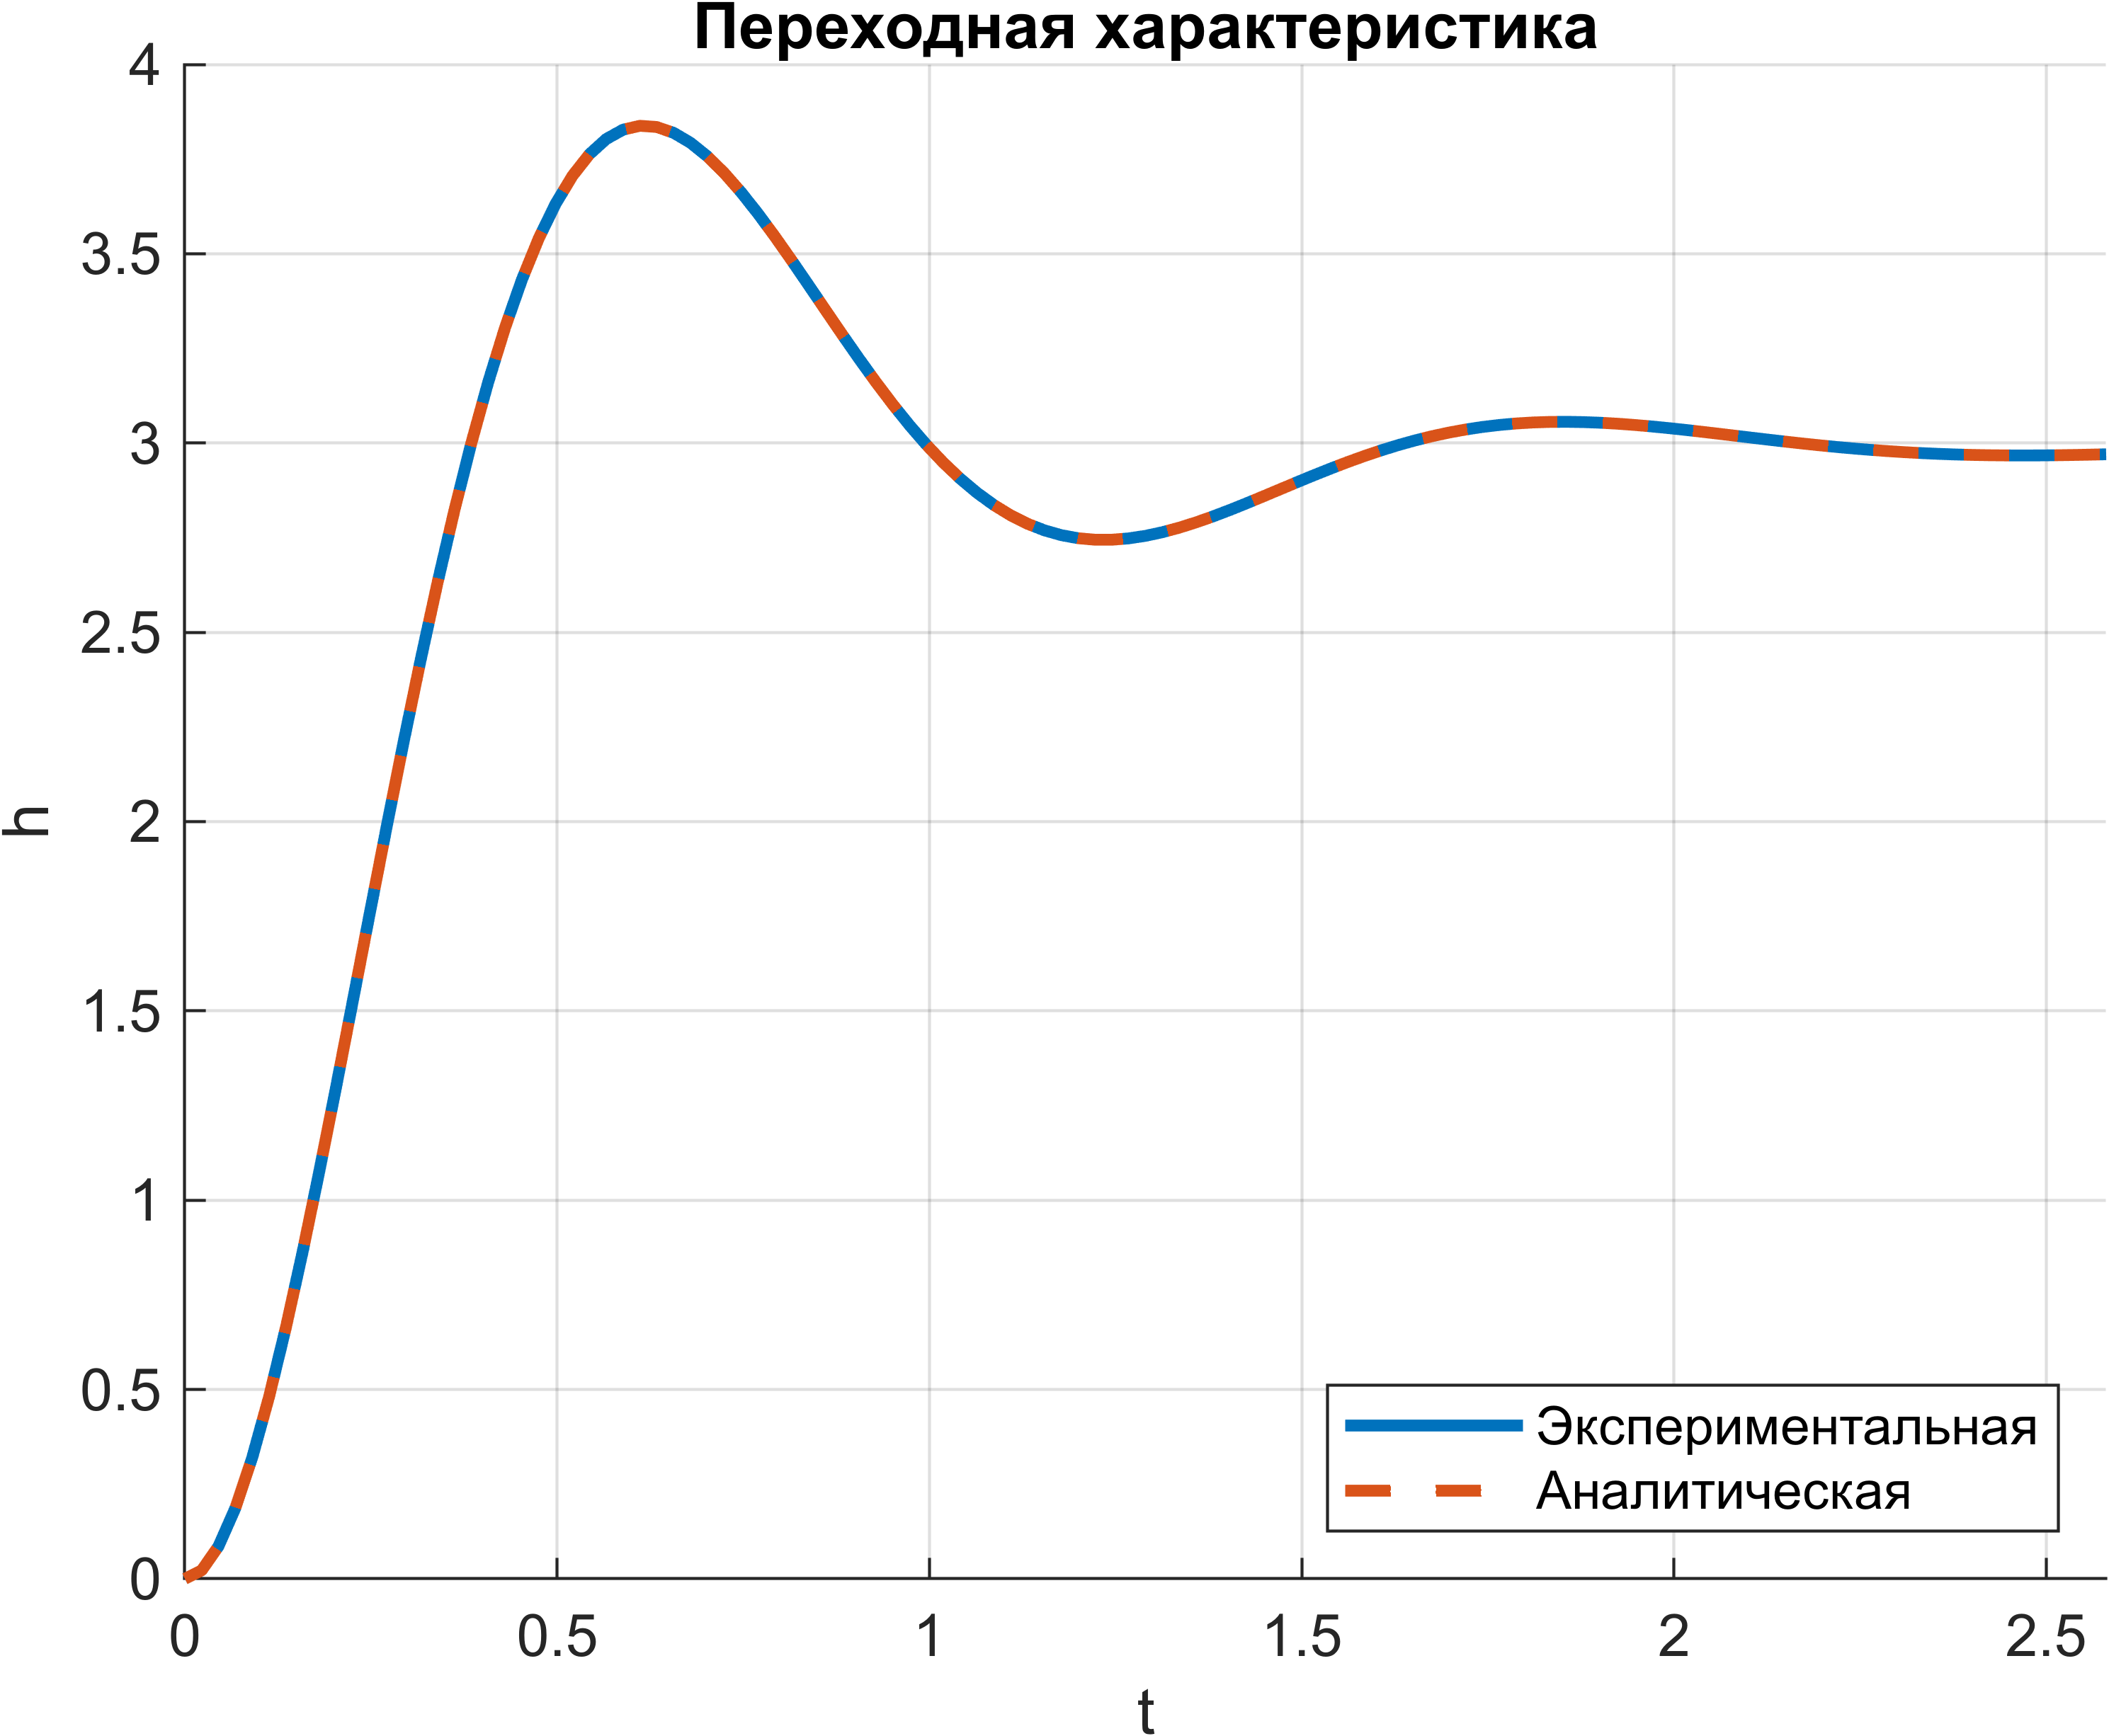
\includegraphics[width=0.75\textwidth, trim={0cm 0cm 0cm 0cm}]{../images/2_1.png}
    \caption{Переходная характеристика полной модели ДПТ} 
\end{figure}

\begin{figure}[H]
    \centering
    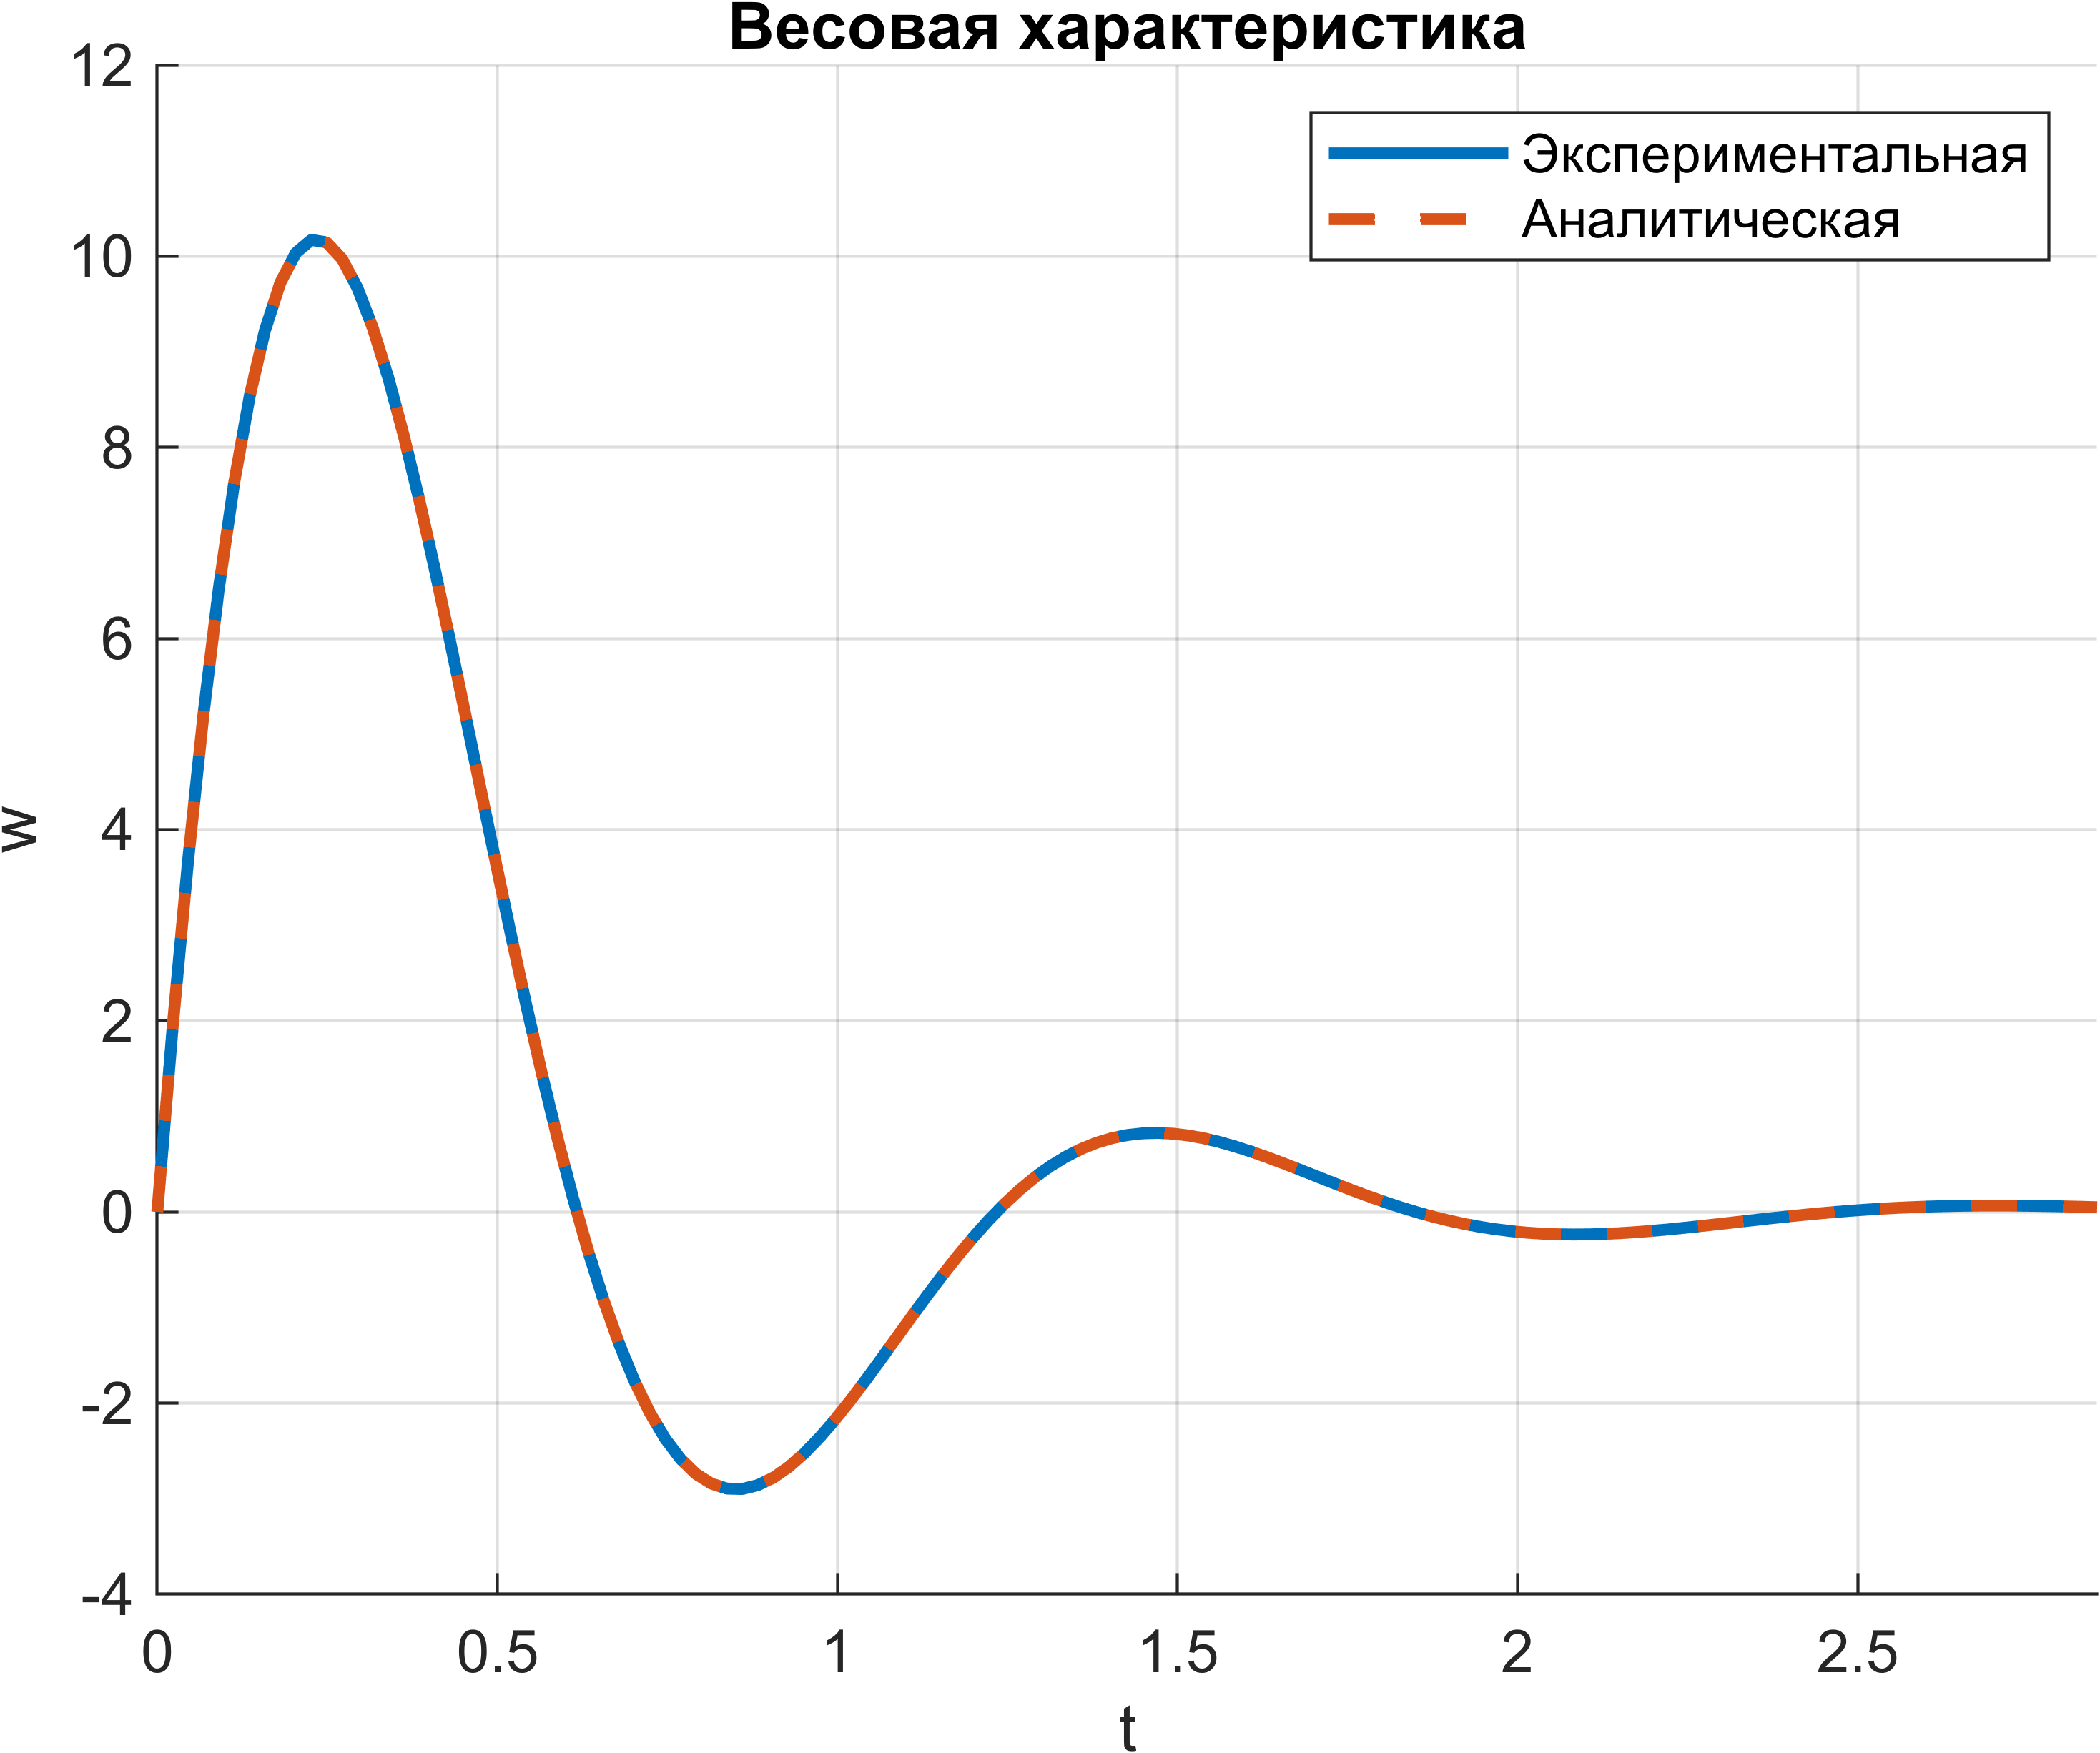
\includegraphics[width=0.75\textwidth, trim={0cm 0cm 0cm 0cm}]{../images/2_2.png}
    \caption{Весовая характеристика полной модели ДПТ}
\end{figure}

\section{Частотные характеристики}

Амплитудно-частотная характеристика для колебательного звена имеет вид:

\[
    A(\omega) = \frac{K}{\sqrt{(1 - \omega^2 T^2)^2 + (2 \xi \omega T)^2}}
\]

Логарифмическая амплитудно-частотная характеристика:
\[
    L(\omega) = 20 \lg(K) - 10 \lg\left((1 - \omega^2 T^2)^2 + 4 \omega^2 \xi^2 T^2\right)
\]

Фазо-частотная характеристика для колебательного звена имеет вид:
\[
    \varphi(\omega) = -a\pi - \arctan\left(\frac{2 \xi \omega T}{1 - \omega^2 T^2}\right), \quad 
    a = 
    \begin{cases} 
    0, & \omega < T^{-1} \\ 
    1, & \omega > T^{-1} 
    \end{cases}
\]

\begin{figure}[H]
    \centering
    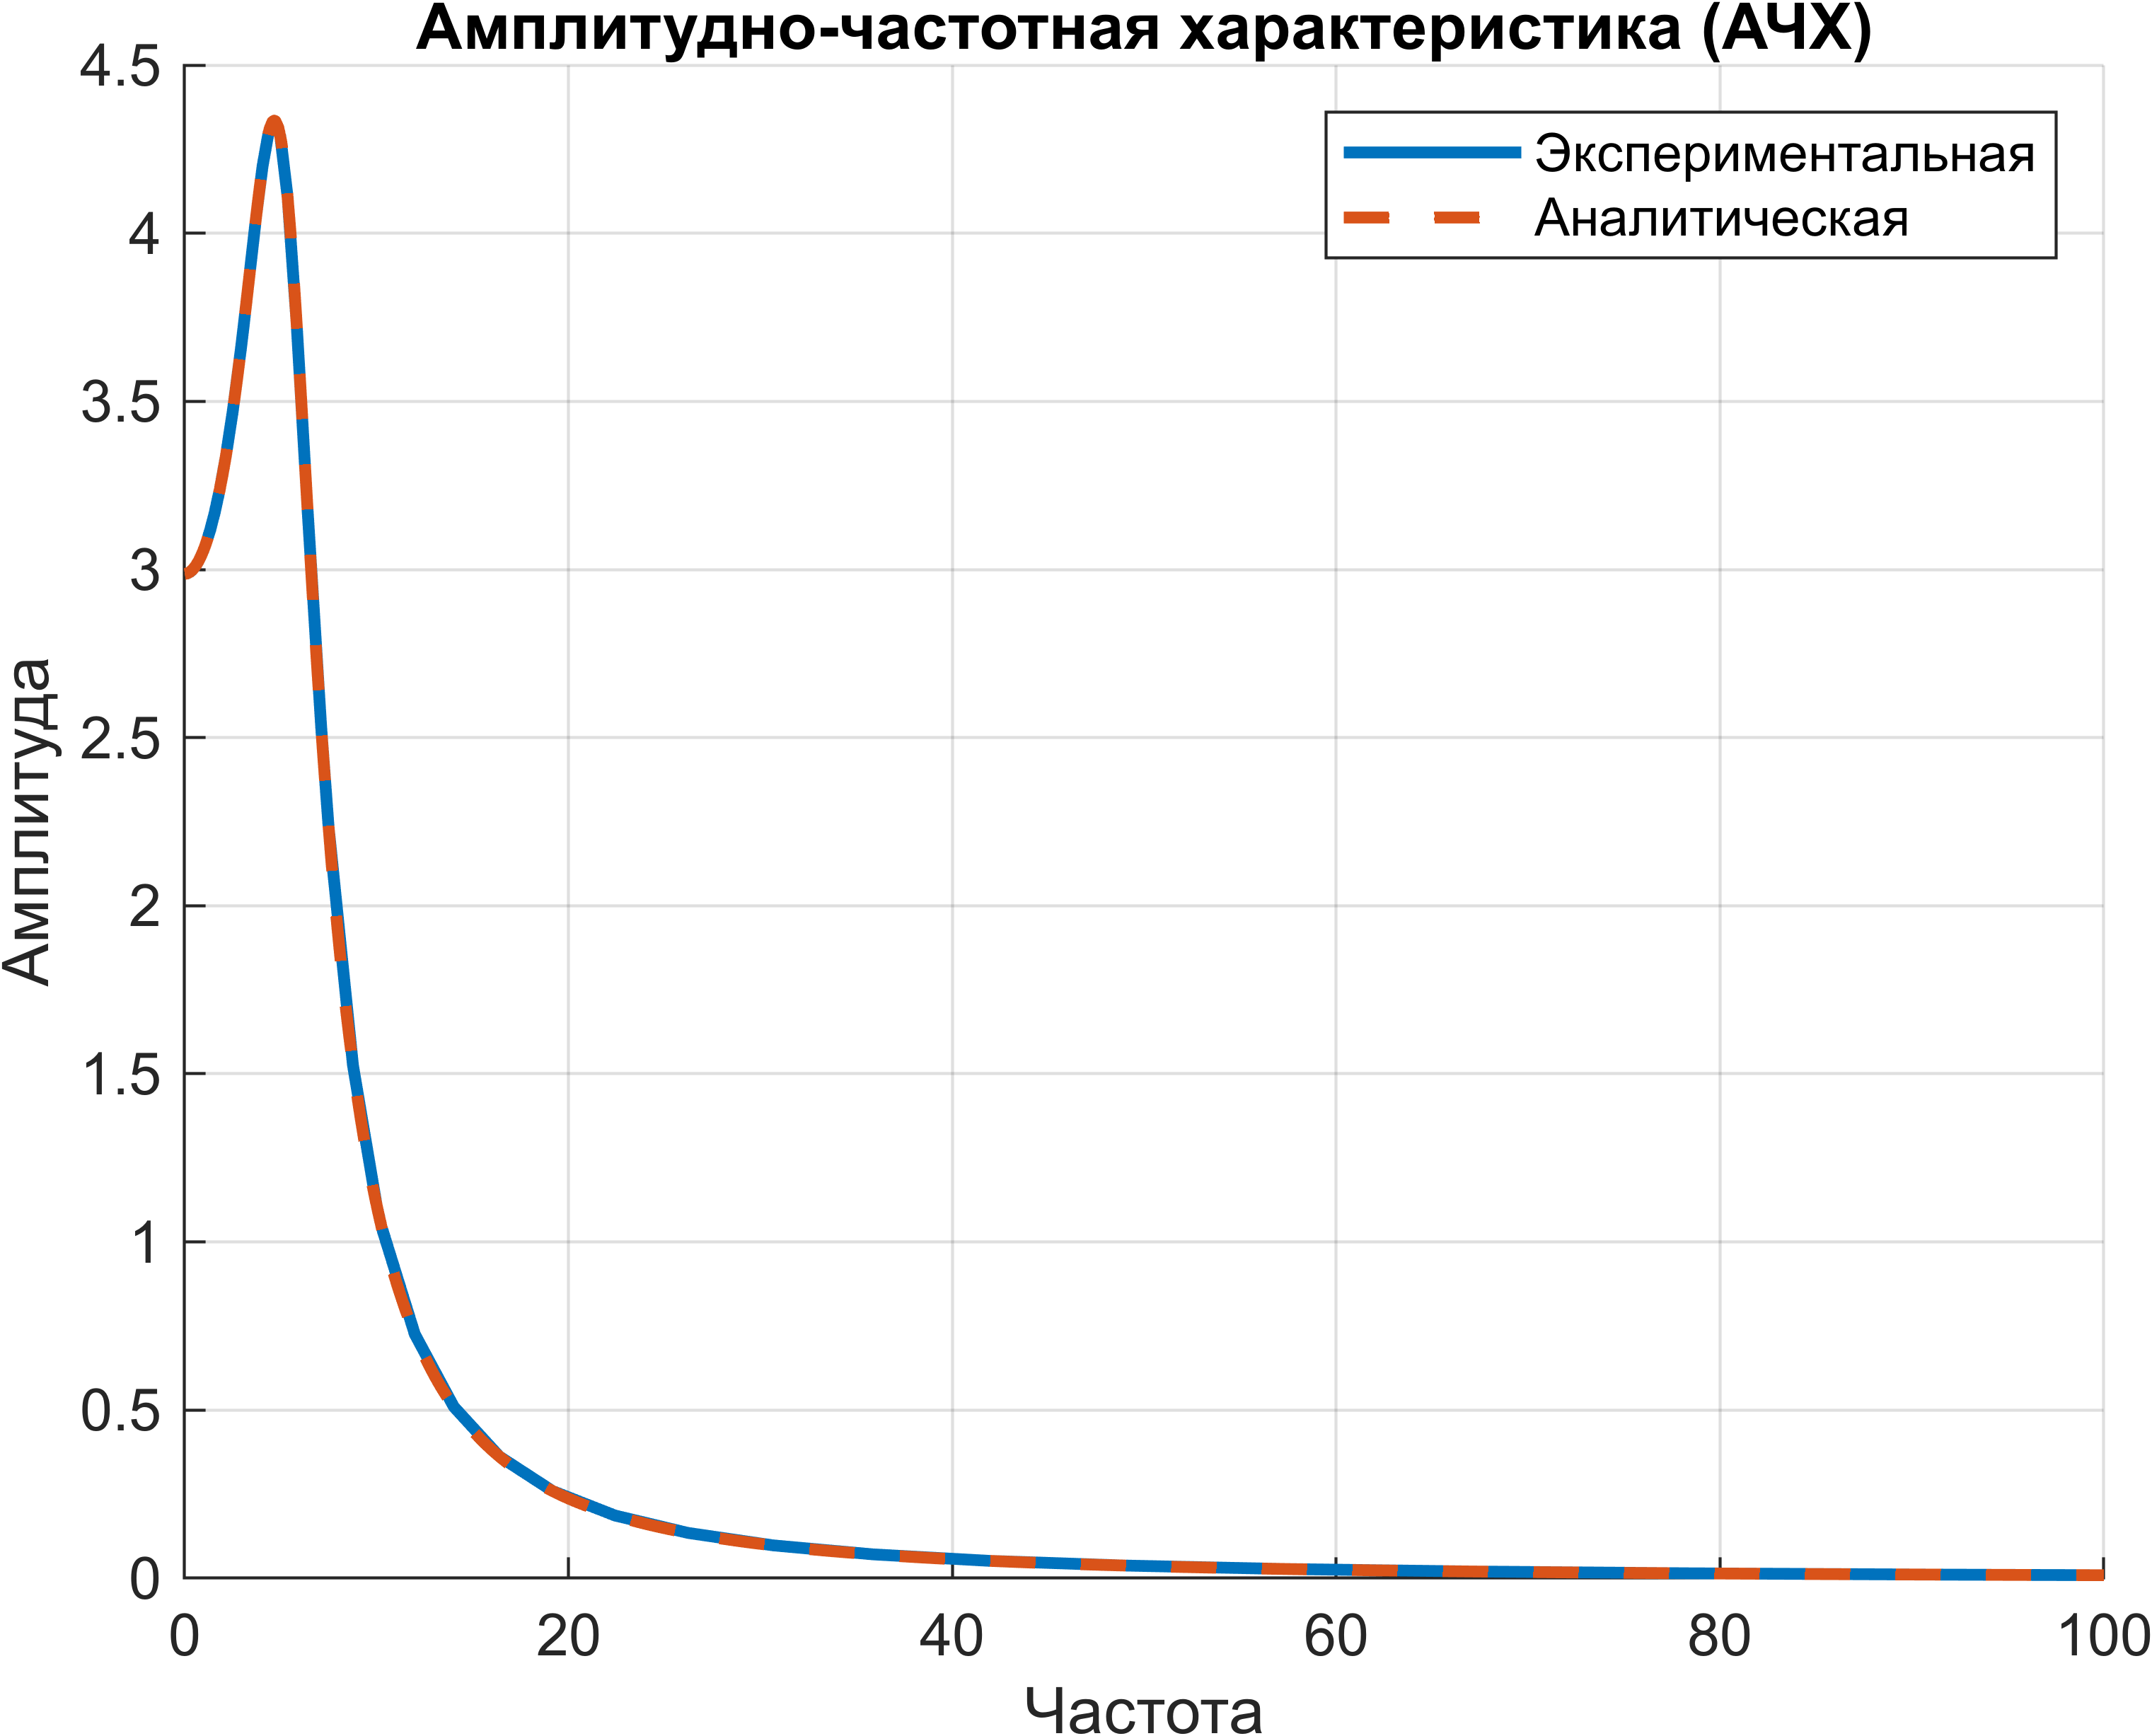
\includegraphics[width=0.75\textwidth, trim={0cm 0cm 0cm 0cm}]{../images/2_3.png}
    \caption{Амплитудно-частотная характеристика полной модели ДПТ}
\end{figure}

\begin{figure}[H]
    \centering
    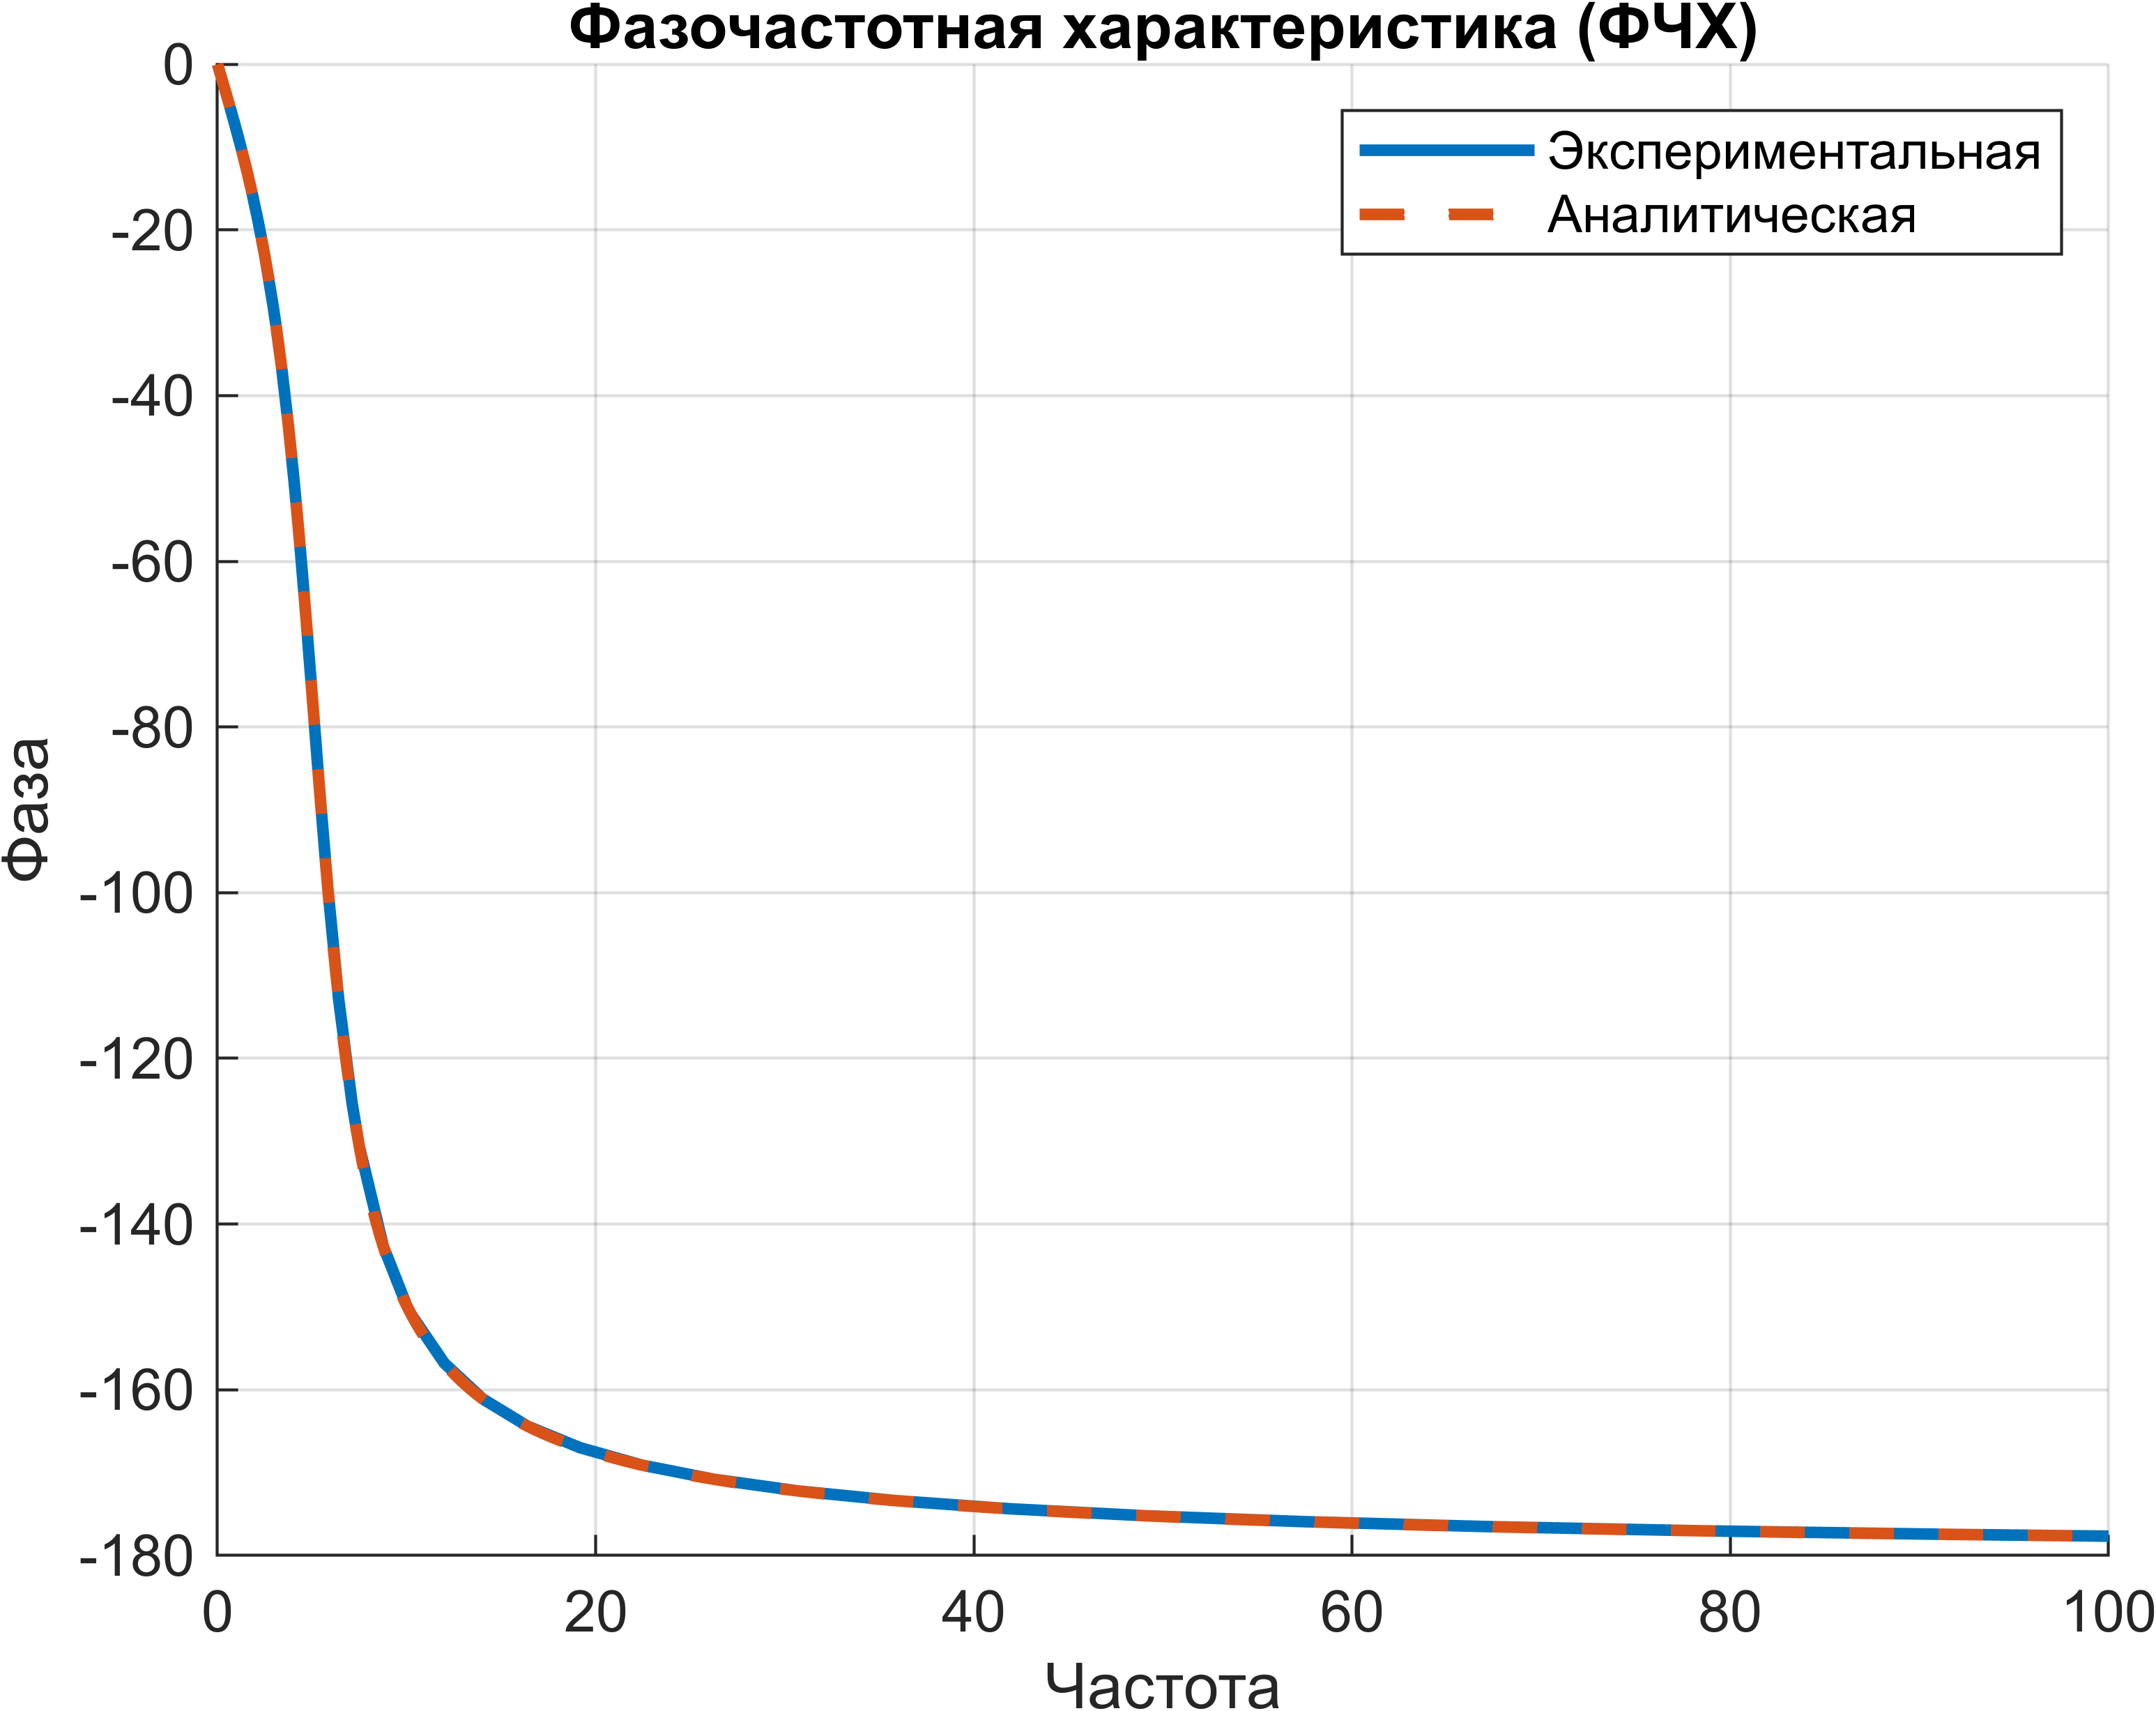
\includegraphics[width=0.75\textwidth, trim={0cm 0cm 0cm 0cm}]{../images/2_4.png}
    \caption{Фазо-частотная характеристика полной модели ДПТ}
\end{figure}

\begin{figure}[H]
    \centering
    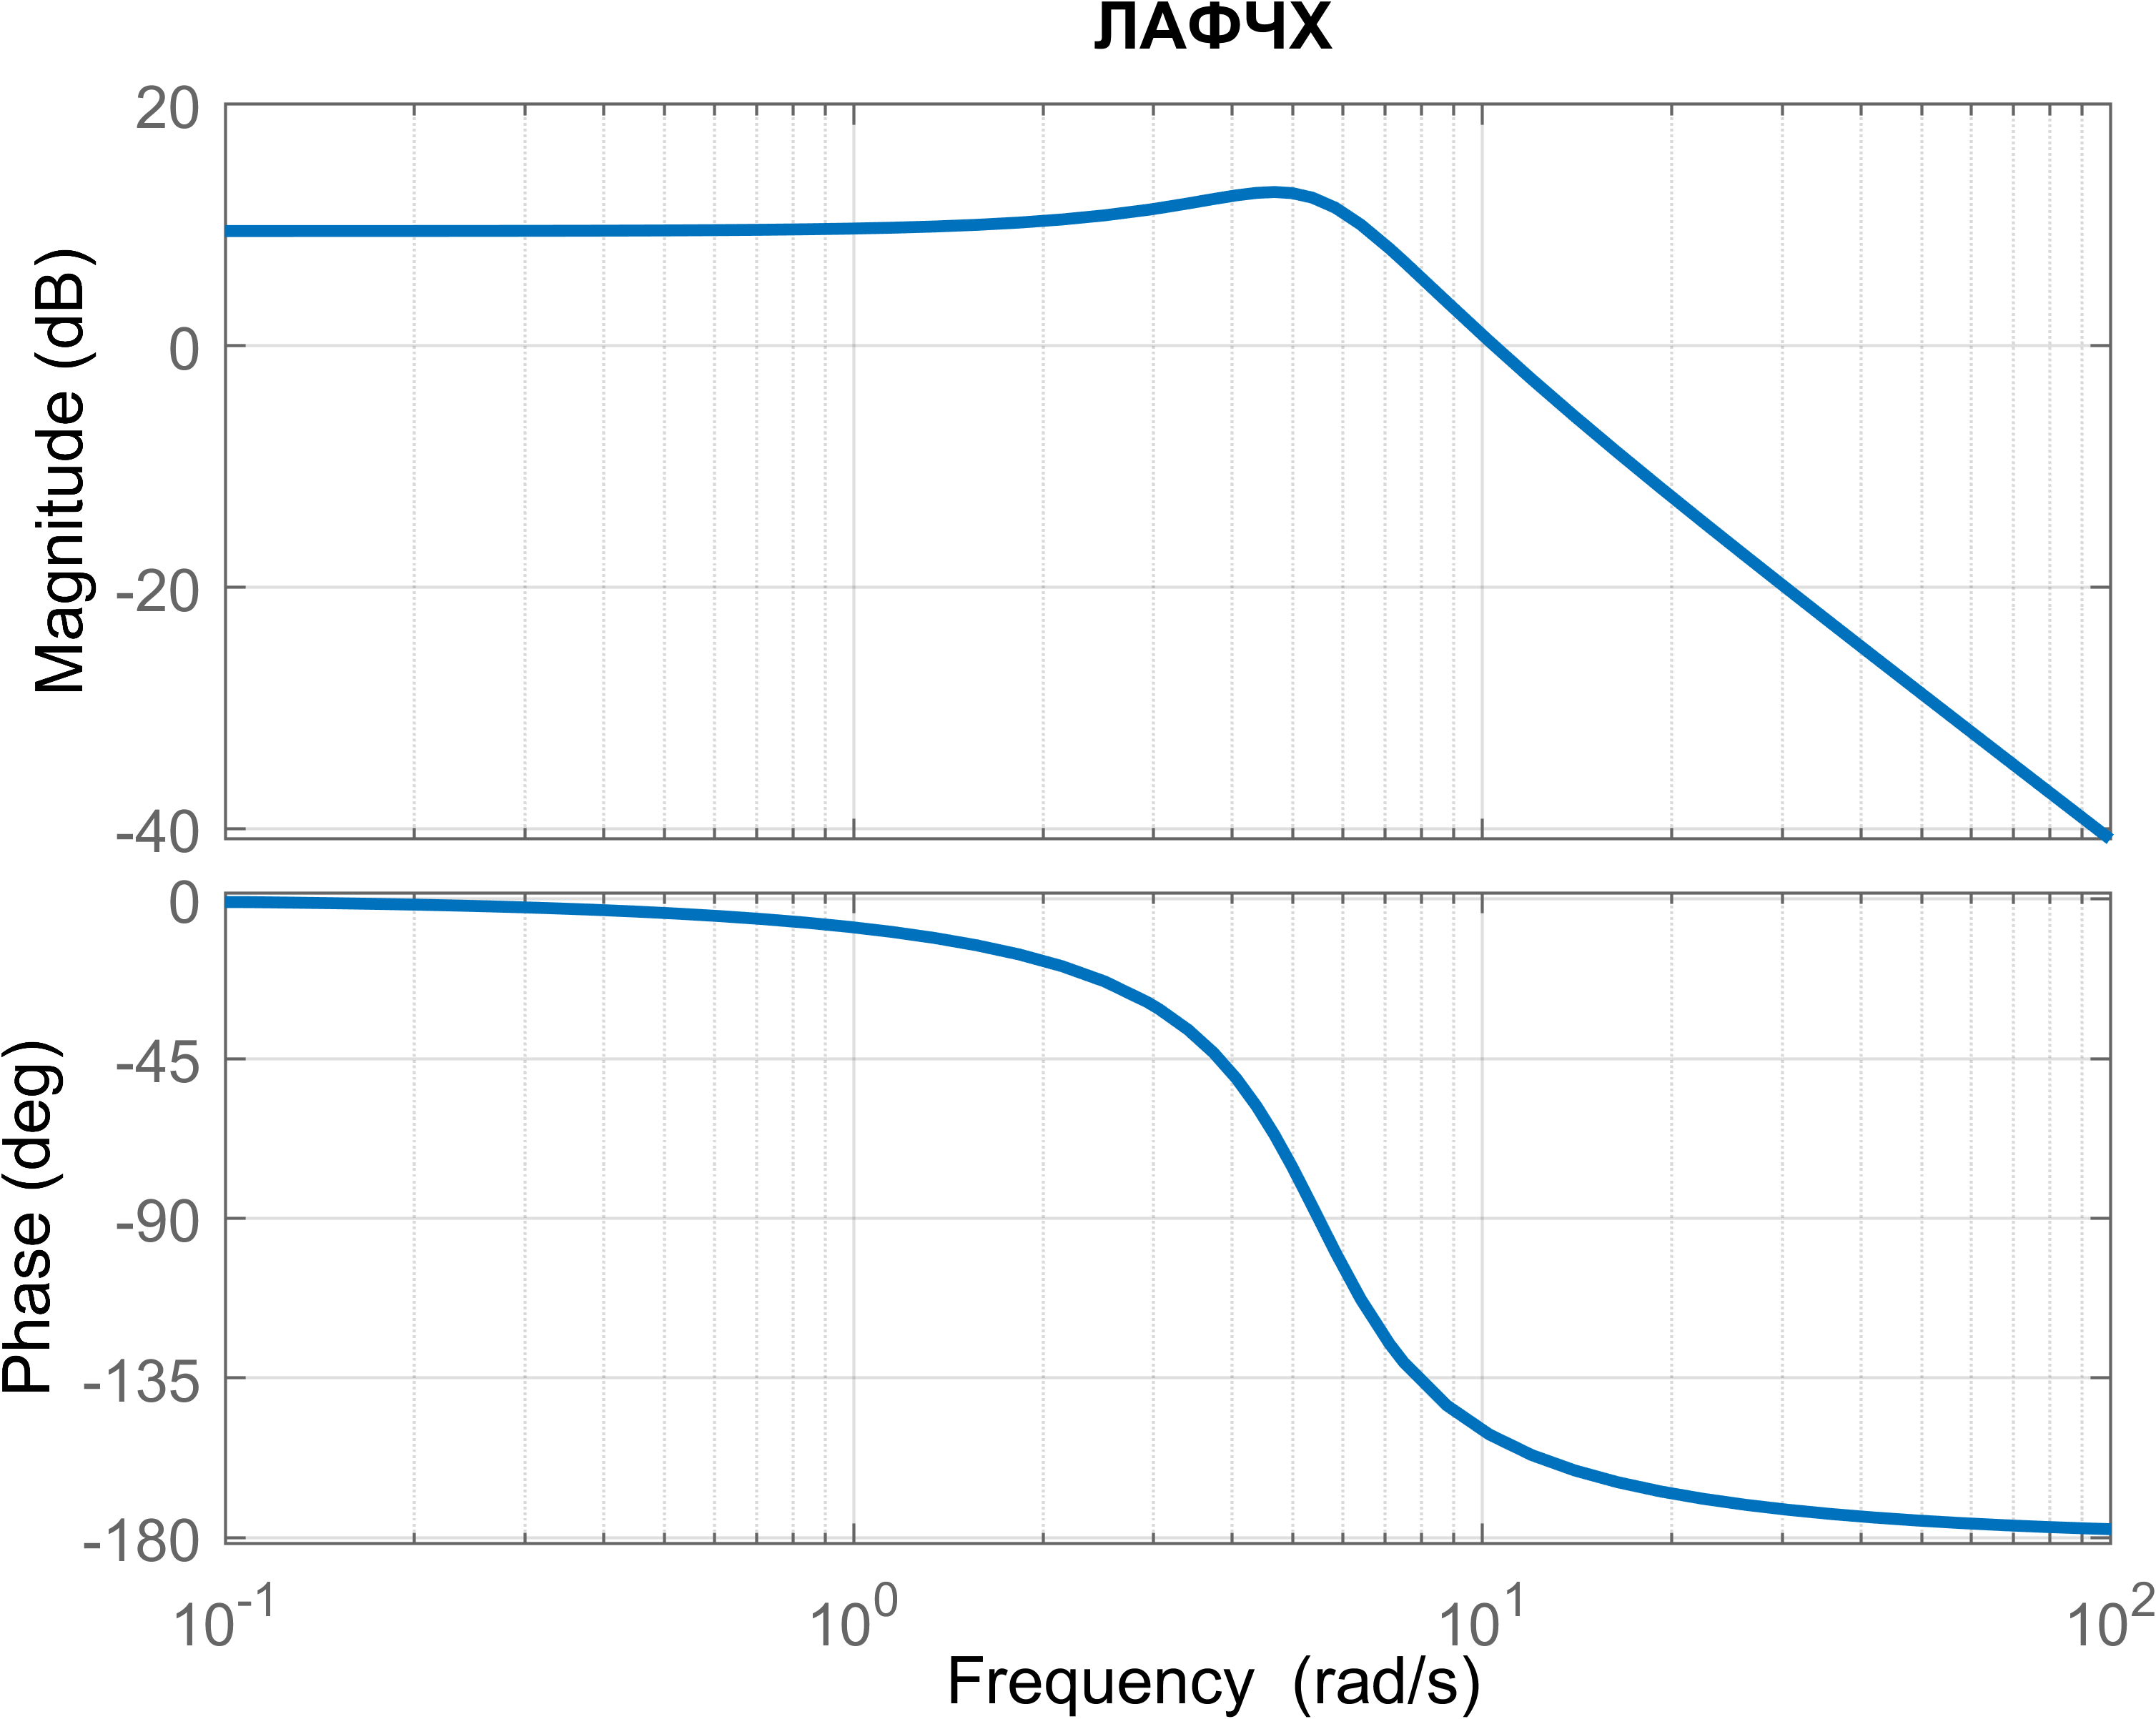
\includegraphics[width=0.75\textwidth, trim={0cm 0cm 0cm 0cm}]{../images/2_5.png}
    \caption{Логарифмическая амплитудно-фазо-частотная характеристика полной модели ДПТ}
\end{figure}

\endinput